\chapter{RNA Secondary Stucture Problem}
\label{chap:rna}

La ricerca della struttura secondaria dell'RNA è un problema a 2
variabili risolvibile tramite il paradigma della programmazione
dinamica. Come sappiamo il DNA è composto da due filamenti, mentre l'RNA
è composto da un filamento singolo. Questo comporta che spesso le basi
di un singolo filamento di RNA si accoppino tra di loro.\\

L'insieme della basi può essere visto come l'alfabeto $\{A, C, U, G\}$
e l'RNA è una sequenza di simboli presi da questo alfabeto.\\

Il processo di accoppiamento delle basi è dettato dalla regola di
\emph{Watson-Crick} e segue il seguente schema:

\begin{center}
  $A-U$ \ \ \ e \ \ \ $C-G$ \ \ \ (l'ordine non conta)
\end{center}


\begin{figure}[H]
  \centering
  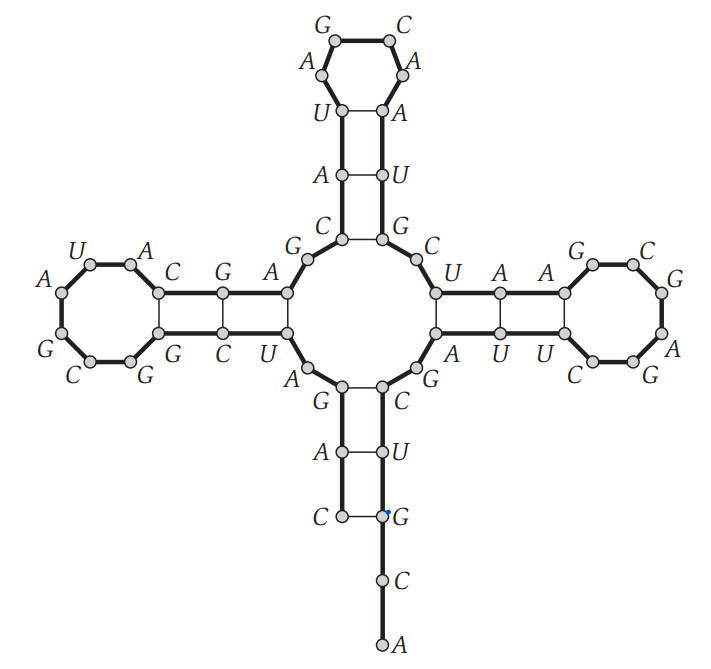
\includegraphics[width=10cm, keepaspectratio]{capitoli/programmazione_dinamica/imgs/rna1.png}
  \caption{Un possibile ripiegamento dell' \textbf{RNA}}
\end{figure}


\textbf{RNA:} stringa $b_0,b_1, \ldots, b_n$ su alfabeto $\{A, C, G, U\}$

\section{Descrizione del Problema}

In questo problema si vuole trovare la struttura secondaria dell'RNA che
abbia \textbf{maggiore energia libera (ovvero il maggior numero di
  coppie di basi possibili)}. Per farlo dobbiamo tenere in considerazione
alcune condizioni che devono essere soddisfatte per permettere di
approssimare al meglio il modello biologico dell'RNA.\\

Formalmente la struttura secondaria di $B$ è un insieme di coppie
$S = \{(i,j)\}$ dove $i,j \in \{1,2,\ldots,n\}$, che soddisfa le
seguenti condizioni:

\begin{enumerate}
  \def\labelenumi{\arabic{enumi}.}
  \item \label{ss:1}
        \textbf{No sharp turns}: la fine di ogni coppia è separata da almeno 4
        basi, quindi se $(i,j) \in S$ allora $i < j - 4$
  \item \label{ss:2}
        Gli elementi di una qualsiasi coppia $S$ consistono di $\{A, U\}$
        o $\{C, G\}$ (in qualsiasi ordine).
  \item
        $S$ è un \textbf{matching}: nessuna base compare in più di una
        coppia.
  \item
        \textbf{Non crossing condition}: se $(i, j)$ e $(k,l)$ sono due
        coppie in $S$ allora \textbf{non può avvenire che}
        $i < k < j < l$.
\end{enumerate}

\begin{figure}[H]
  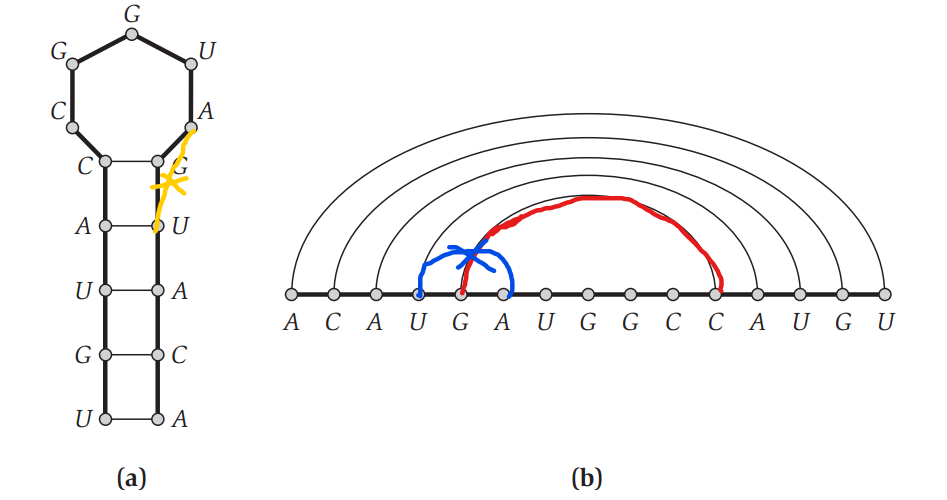
\includegraphics[width=\textwidth, keepaspectratio]{capitoli/programmazione_dinamica/imgs/rna2.png}
  \centering
  \caption{La figura $(a)$ rappresenta un esempio di Sharp Turn, mentre la
    figura $(b)$ mostra una Crossing Condition dove il filo blu non dovrebbe
    esistere.}
\end{figure}

\subsection{Goal}

Data una molecola di RNA trovare una struttura secondaria che massimizza
il numero di coppie.

\section{Funzionamento}

Per mappare il problema sul paradigma della programmazione dinamica,
come prima idea, potremmo basarci sul seguente sotto-problema:
\begin{myblockquote}
  \begin{itemize}
    \item Affermiamo che $OPT(j)$ è il massimo numero di coppie
          di basi sulla struttura secondaria $b_1 b_2 \ldots b_j$
    \item per la Non Sharp Turn Condition sappiamo che
          $OPT(j) = 0$ per $j \leq 5$
    \item e sappiamo anche che
          $OPT(n)$ è la soluzione che vogliamo trovare.
  \end{itemize}
\end{myblockquote}


Il problema sta nell'esprimere $OPT(j)$ ricorsivamente. Possiamo
parzialmente farlo sfruttando le seguenti scelte:
\begin{enumerate}
  \item $j$ non appartiene ad una coppia
  \item $j$ si accoppia con $t$ per qualche $t \leq j - 4$
\end{enumerate}

Per il primo caso basta cercare la soluzione per $OPT(j - 1)$.\\
Nel secondo caso, se teniamo conto della \textbf{Non Crossing
  Condition}, possiamo isolare due nuovi sotto-problemi: uno sulle basi
$b_1 b_2 \ldots b_{t-1}$ e l'altro sulle basi
$b_{t+1} \ldots b_{j-1}$.

\begin{itemize}
  \item
        Il primo si risolve con $OPT(t-1)$
  \item
        Il secondo, dato che non inizia con indice $1$, non è nella lista
        dei nostri sotto-problemi. A causa di ciò risulta necessario
        aggiungere una variabile.
\end{itemize}

\begin{figure}[H]
  \centering
  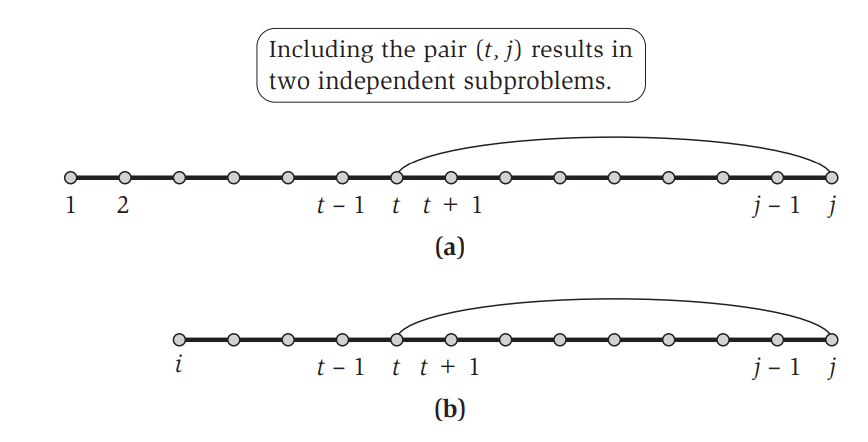
\includegraphics[width=\textwidth, keepaspectratio]{capitoli/programmazione_dinamica/imgs/rna3.png}
  \centering
\end{figure}


Basandoci sui ragionamenti precedenti, possiamo scrivere
una ricorsione di successo, ovvero:\\

sia $OPT(i,j)$ il massimo numero di coppie nella
struttura secondaria $b_i b_{i+1} \ldots b_j$, grazie alla \textbf{non
  Sharp turn Condition} possiamo inizializzare gli elementi con
$i \geq j -4$ a $0$. Ora avremmo sempre le stesse condizioni
elencate sopra:
\begin{itemize}
  \item $j$ non appartiene ad una coppia
  \item $j$ si accoppia
        con $t$ per qualche $t \leq j - 4$
\end{itemize}

Nel primo caso avremmo che $OPT(i,j) = OPT(i, j-1)$, nel secondo caso
possiamo ricorrere su due sotto-problemi $OPT(i, t-1)$ e
$OPT(t+1, j-1)$ affinché venga rispettata la \textbf{non crossing
  condition}.\\

Riassumendo, distinguiamo 3 diversi casi:
\begin{enumerate}
  \item se $i \ge j -4$:\\
        $OPT(i,j) = 0$ dalla \textbf{no-Sharp Turns condition}
  \item $b_j$ non viene accoppiata:\\ $OPT(i,j) = OPT(i,j-1)$
  \item $b_j$ si accoppia con $b_t$ per una qualche $i \le t < j -4$:\\
        $OPT(i,j) = 1 + \max_t(OPT(i, t-1) + OPT(t+1, j-1))$
\end{enumerate}


Possiamo esprimere formalmente la ricorsione come segue:
\\
\begin{myblockquote}
  $OPT(i, j) = \max(OPT(i, j-1), \max_t(1+OPT(i, t-1)+OPT(t+1, j-1)))$,\\
  dove il massimo è calcolato su $t$ tale che $b_t$ e
  $b_j$ siano una coppia di basi consentita (sotto le condizioni (\ref{ss:1}) e
  (\ref{ss:2}) dalla definizione di struttura secondaria).
\end{myblockquote}



\begin{figure}[H]
  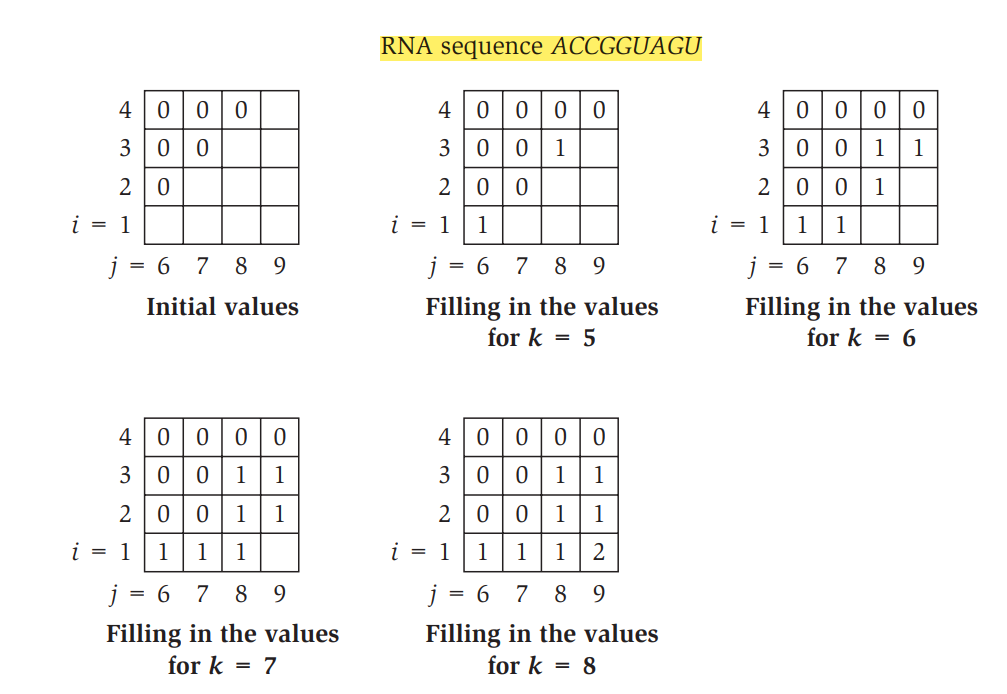
\includegraphics[width=12cm, keepaspectratio]{capitoli/programmazione_dinamica/imgs/rna4.png}
  \centering
  \caption{Iterazioni dell'algoritmo su un campione del problema in
    questione $(ACCGGUAGU)$}
\end{figure}


Possiamo infine formalizzare il tutto con il seguente pseudo-codice:

\begin{lstlisting}[language=Python, mathescape=true]
  Initialize-OPT(i, j) = 0 whenever i $\le$ j - 4

  for k = 5 to n - 1 
	  for i = 1 to n - k
		  j $\leftarrow$ i + k
		  Compute M[i, j] using the previous recurrence formula
  return M[1,n]
\end{lstlisting}

\subsection{Costo}

Ci sono $O(n^2)$ sotto-problemi da risolvere e ognuno richiede tempo
$O(n)$, quindi il running time complessivo è di $O(n^3)$.\\

Costo computazionale:
\begin{itemize}
  \item \textbf{Tempo:} $O(n^3)$
  \item \textbf{Spazio:} $O(n^2)$
\end{itemize}

\section{Riepilogo}

\begin{itemize}
  \item
        Trovare il modo di accoppiare le basi di RNA con delle regole
  \item
        $OPT[i,j] = \max(\max_{i \le t \le j-5}(1 + OPT[i, t-1] + OPT[t+1, j-1]), OPT[i, j-1])$
  \item
        Spazio = matrice riempita per diagonali $\rightarrow$ \textbf{SPAZIO
          =} $O(n^2)$
  \item
        Per calcolare ogni $OPT$ pago $n$ $\rightarrow$ \textbf{TEMPO =}
        $O(n^3)$
  \item
        Per costruire una soluzione mi serve una matrice dove
        $S[i,j] = \max_t$ $\rightarrow$ \textbf{SPAZIO =} $O(n^2)$
\end{itemize}
